\documentclass[]{article}
\usepackage[utf8]{inputenc}
\usepackage[T1]{fontenc}
\usepackage[total={11in,8.5in},portrait,left=1in,right=1in,top=1.5in]{geometry}
\usepackage{amsmath}
\usepackage{amsfonts}
\usepackage{textgreek}
\usepackage{graphicx}
\usepackage{hyperref}
\begin{document}
\title{BMI 203 HW 3}
\author{Garrett Wong}
\date{22 February 2019}
\maketitle

Code, including optimized matrices, is at \url{https://github.com/garrett-wong/BMI203_HW3}.

\section{Optimizing gap penalites}

\subsection{Consider the false positive rate (proportion of negative pairs with scores that exceed a score threshold) when the true positive rate (proportion of positive pairs with scores above the threshold) is 0.7. What's the best false positive rate that you can achieve with varying both gap opening (from 1 to 20) and extension penalties (from 1 to 5) with the BLOSUM50 matrix? What is the best gap penalty combination?}

I varied the gap opening penalty and extension penalties from 1 to 20 and 1 to 5 with the BLOSUM50 matrix and found the following pattern of FP rates when the TP rate was controlled to 0.7: (darker blue indicates a better(lower) false positive rate)

\vspace{1em}
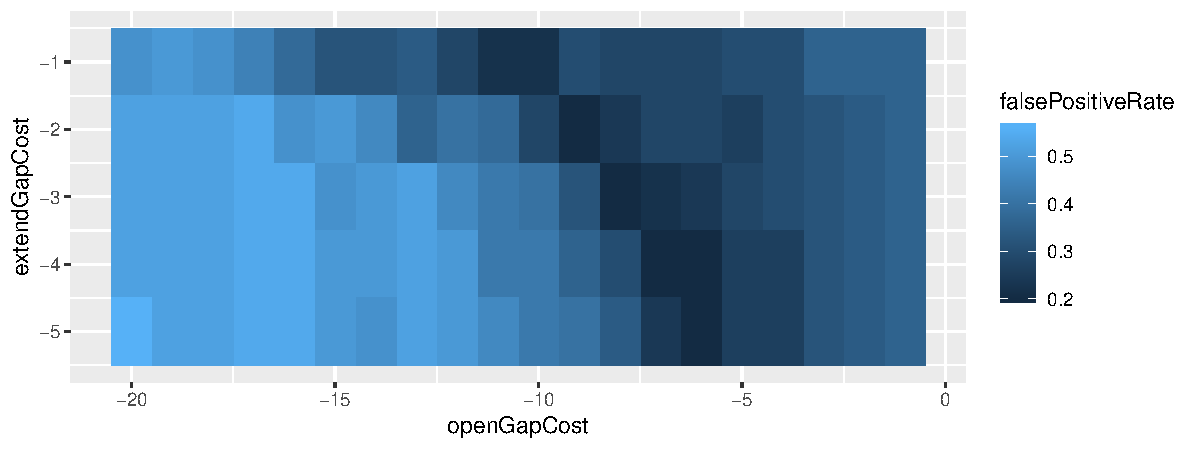
\includegraphics[width=\textwidth]{../BMI203_HW3_alignment/plots/optimizeGapPenalties.pdf}
\vspace{1em}

We can see a diagonal of optimal gap opening and extension penalties, with penalties of (-6, -5), (-6, -4), (-7, -4), (-8, -3), and (-9, -2) respectively; all sharing the best FP rate of 0.2.

This diagonal pattern indicates a compensatory relationship between the gap opening and extension penalties that makes sense.

\subsection{Using the gap penalties you determined from question 1, which of the provided scoring matrices performs the best, in terms of false positive rate (at a true positive rate of 0.7)? What are the performance rates of each of the matrices? Create a Receiver Operator Curve (ROC) graph which shows the fraction of true positives on the Y axis and the fraction of false positives on the X axis.}

I proceeded with a gap opening penalty of -7 and gap extension penalty of -4. I created a ROC graph for BLOSUM50, which shows the highest AUC among the provided matrices of 0.84:

\vspace{1em}
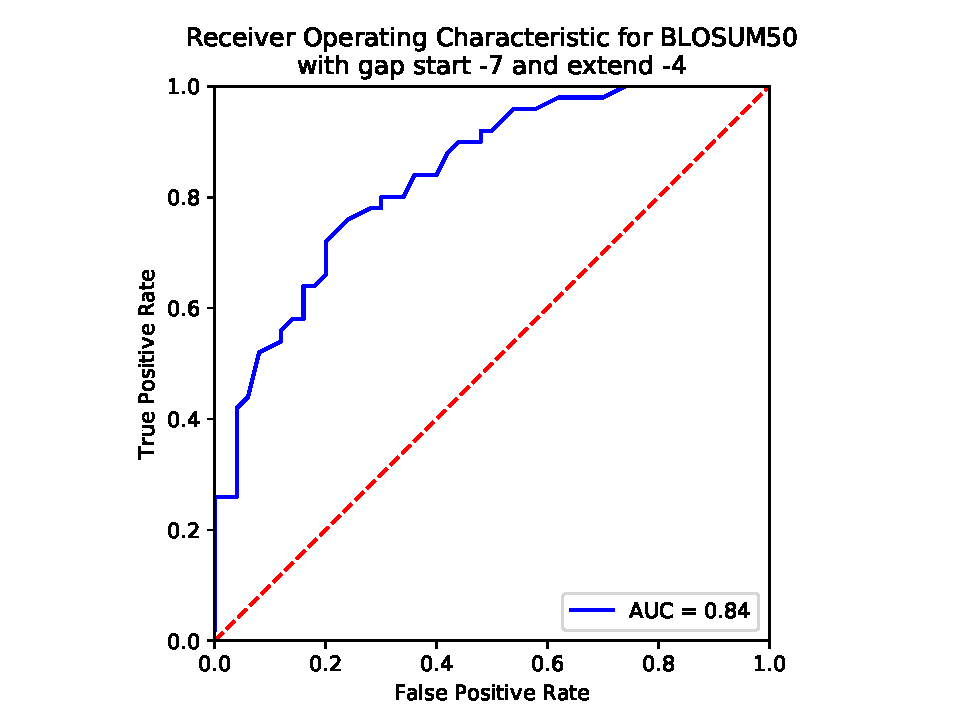
\includegraphics[width=0.5\textwidth]{../BMI203_HW3_alignment/plots/ROC_blosum50.pdf}
\vspace{1em}

compared to the ROC graphs for BLOSUM62, PAM100, PAM250, and MATIO, with AUCs of 0.72, 0.72, 0.82, and 0.70 respectively:

\vspace{1em}
\includegraphics[width=0.5\textwidth]{../BMI203_HW3_alignment/plots/ROC_blosum62.pdf}
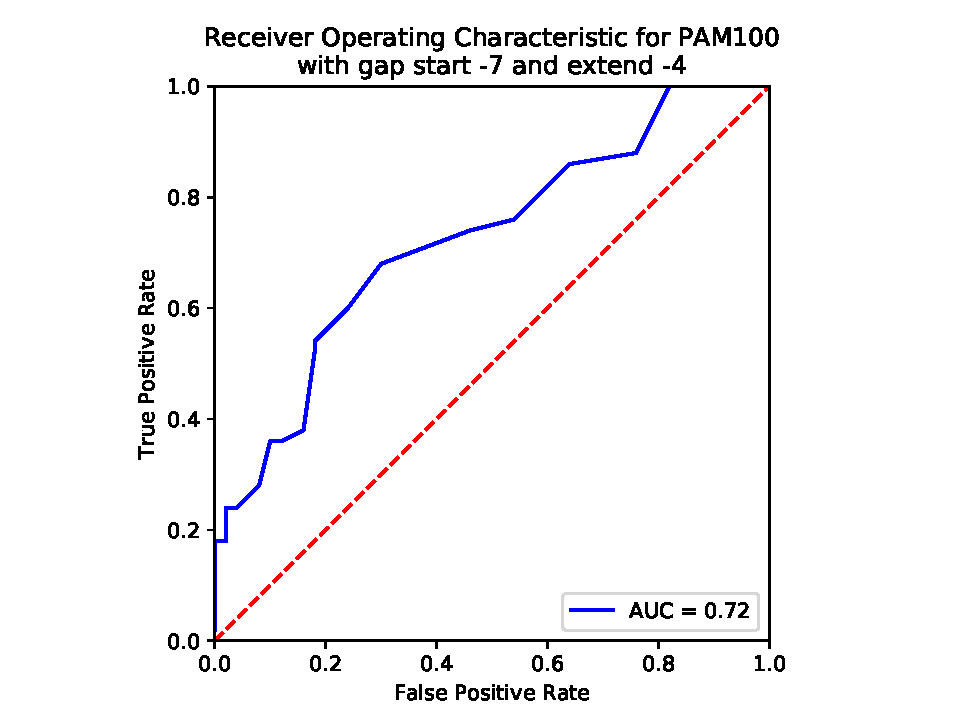
\includegraphics[width=0.5\textwidth]{../BMI203_HW3_alignment/plots/ROC_PAM100.pdf}
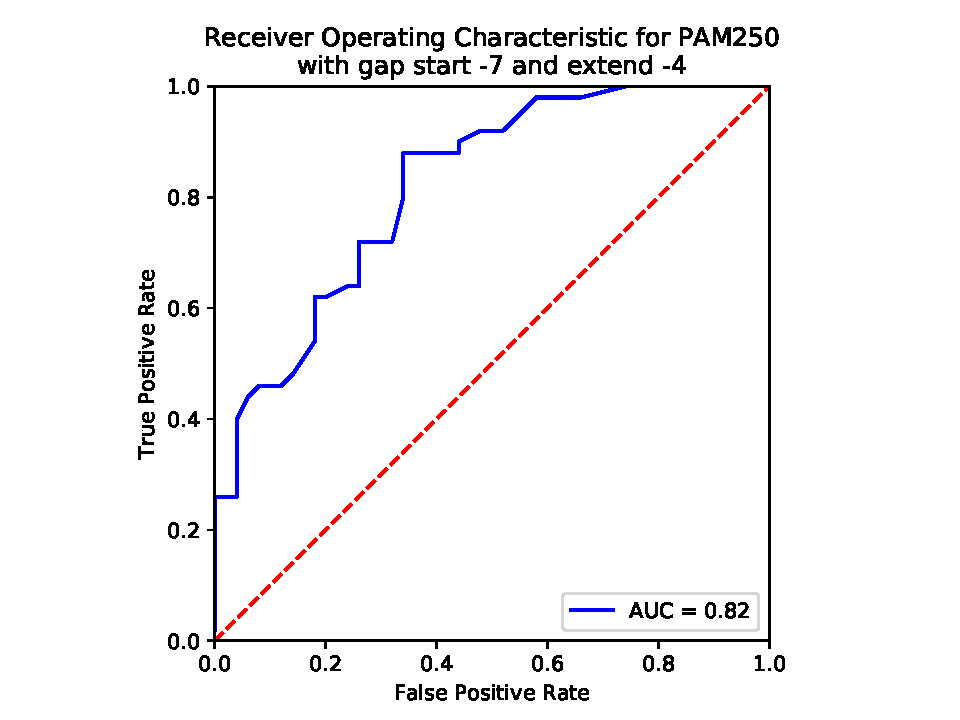
\includegraphics[width=0.5\textwidth]{../BMI203_HW3_alignment/plots/ROC_PAM250.pdf}
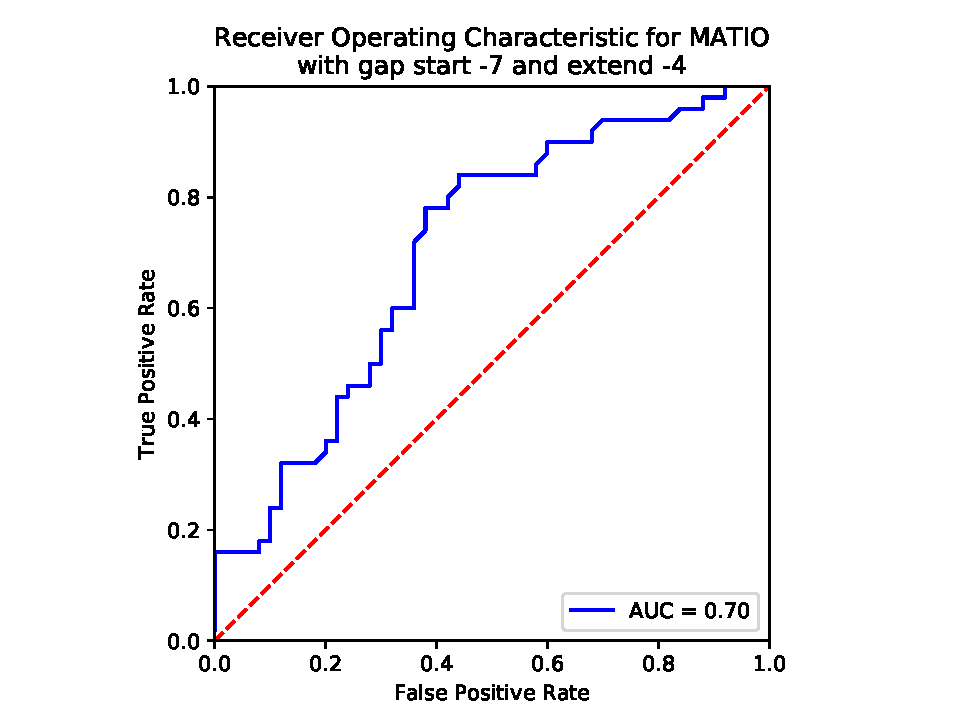
\includegraphics[width=0.5\textwidth]{../BMI203_HW3_alignment/plots/ROC_MATIO.pdf}
\vspace{1em}


\subsection{How does the performance change if you normalize the Smith-Waterman scores by the length of the shortest sequence in a pair (i.e. divide the raw score by the min length)? Show the ROC curves for your best matrix and for the same matrix with normalized scores. Are the false positive rates better or worse? Why do you think this is so?}

When we normalize the Smith-Waterman scores by the length of the shortest sequence in the pair, we see the ROC curves get much worse. For the best performing matrix, BLOSUM50, we can see the AUC of 0.84 drops to 0.5:

\vspace{1em}
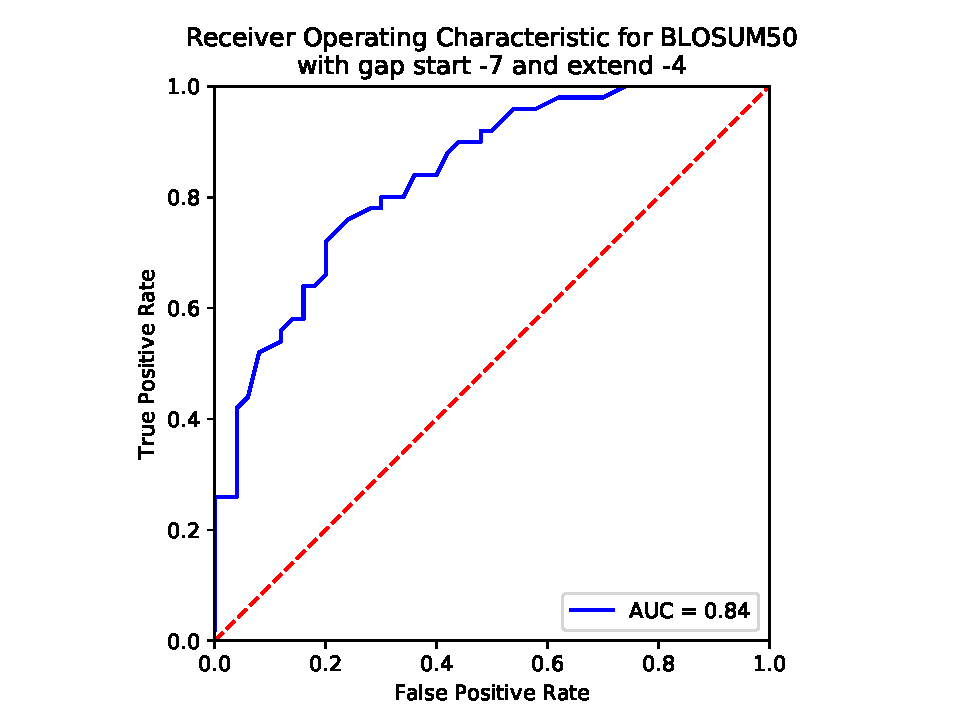
\includegraphics[width=0.5\textwidth]{../BMI203_HW3_alignment/plots/ROC_blosum50.pdf}
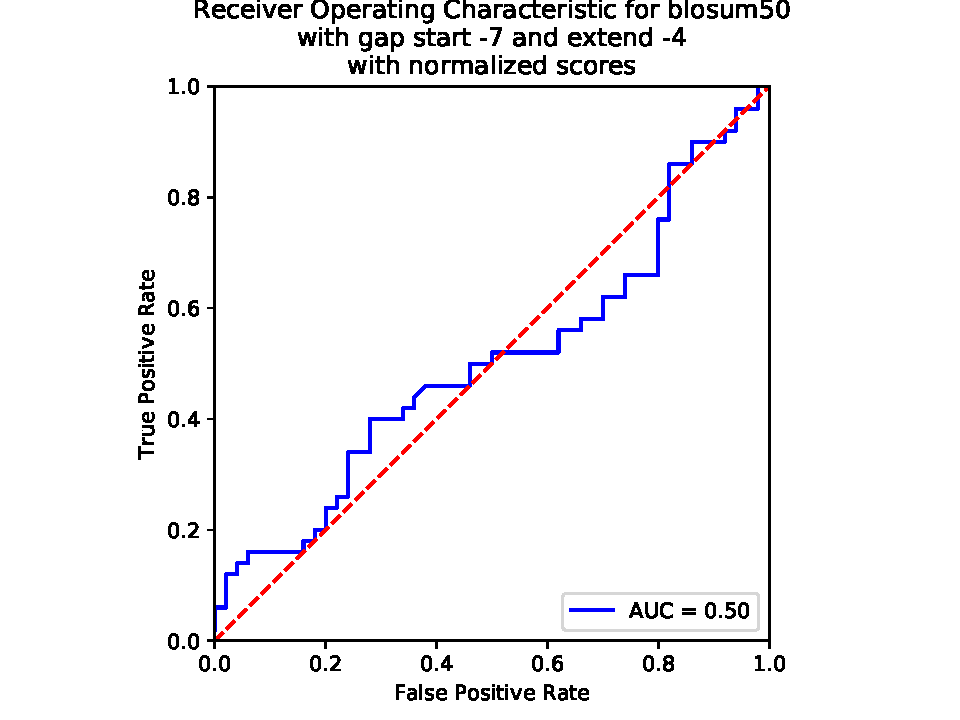
\includegraphics[width=0.5\textwidth]{../BMI203_HW3_alignment/plots/ROC_normScores_blosum50.pdf}
\vspace{1em}

This may be because the normalization doesn't do a good job of capturing the length of the aligning sequence; we might want to, instead, normalize by the length of the aligned section.

\section{Optimizing scoring matrices}
\setcounter{subsection}{1}
\subsection{Beginning from the best matrix from above (that which produced the alignments), run your optimization algorithm to maximize the fitness of the new matrix. How much improvement do you see in the fitness? Show the full ROC curves for the original matrix and the optimized matrix. What happens when you now realign the sequences using the new matrix and rescore? Show the new ROC curve following realignment on the same graph as above. Qualitatively discuss how your matrix and your alignments change following optimization.}

I calculated optimal alignments using BLOSUM50, a gap opening penalty of -7 and gap extension penalty of -4. Optimization of the scoring matrix using a genetic algorithm improved the objective function from 2.16 to 3.76. The ROC curve of this optimized scoring matrix showed an AUC of 0.97:

\vspace{1em}
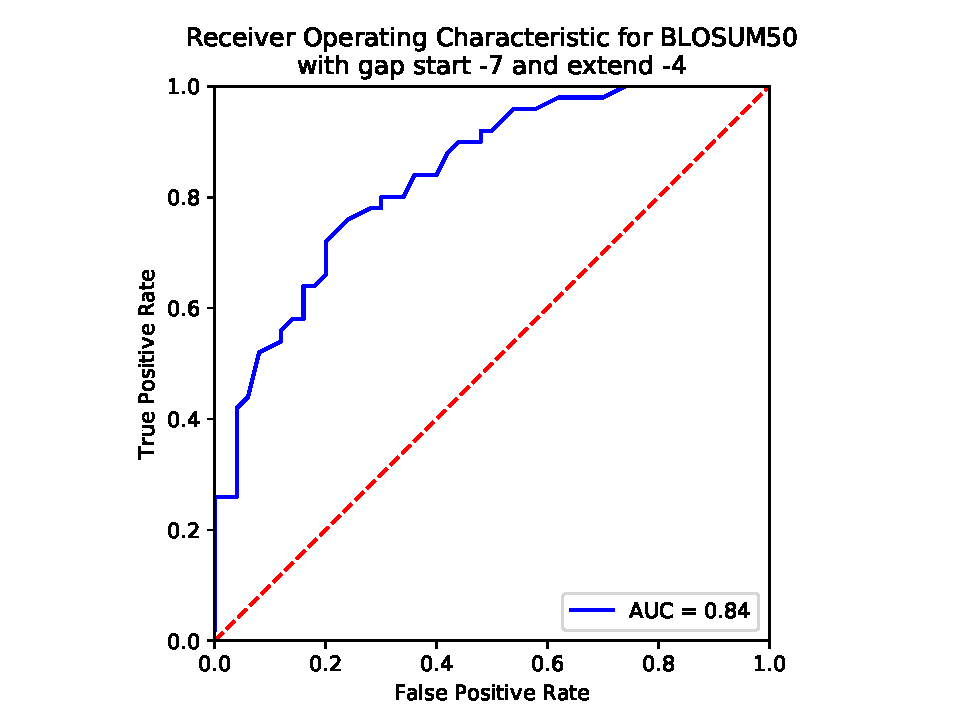
\includegraphics[width=0.5\textwidth]{../BMI203_HW3_alignment/plots/ROC_blosum50.pdf}
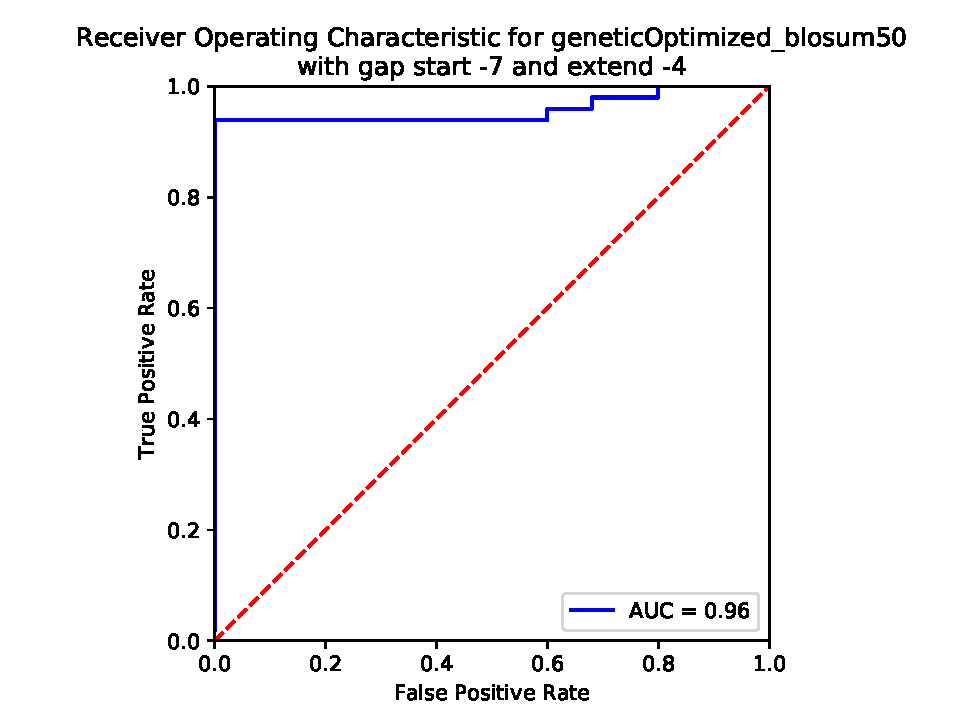
\includegraphics[width=0.5\textwidth]{../BMI203_HW3_alignment/plots/ROC_geneticOptimized_blosum50.pdf}
\vspace{1em}

However, realigning and rescoring indicates a much less impressive ROC curve, with an AUC incidentally equal to the original matrix, at 0.84: 

\vspace{1em}
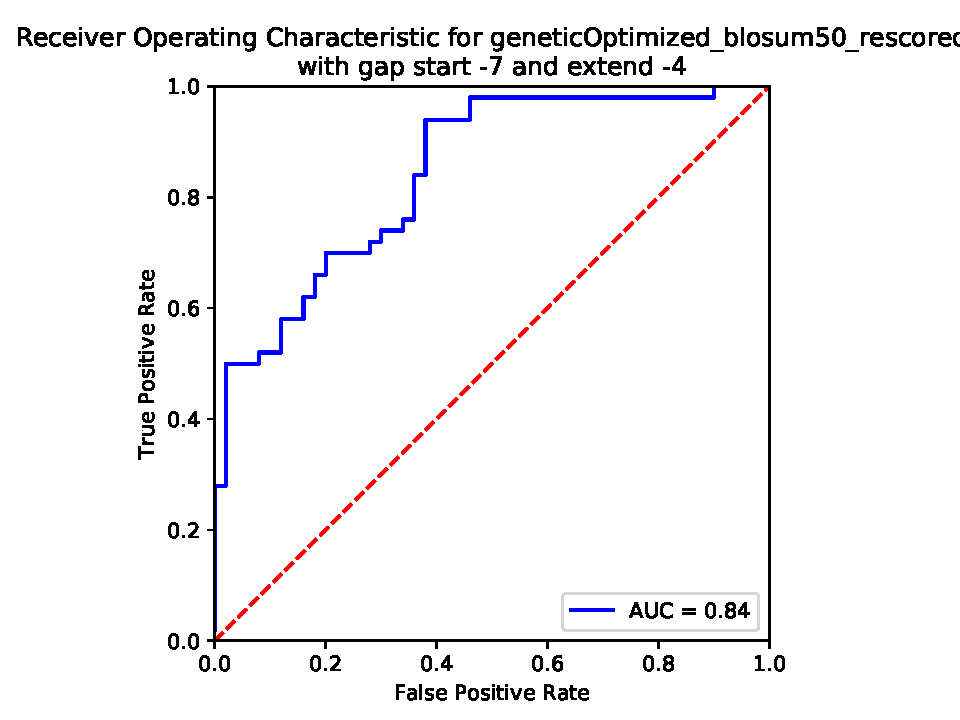
\includegraphics[width=0.5\textwidth]{../BMI203_HW3_alignment/plots/ROC_geneticOptimized_blosum50_rescored.pdf}
\vspace{1em}

This indicates that my optimization algorithm was overfitting on features of the static alignments that we were optimizing on.

\subsection{Beginning from the MATIO matrix, but using the same initial sequence alignments, re-run the optimization. Show the same ROC plots as for (2). Discuss the relationship between the results you see here and the results you saw for (2).}

Optimization of the MATIO scoring matrix on the BLOSUM50 alignments using a genetic algorithm improved the objective function from 0.48 to 2.82 in the final optimized scoring matrix. The ROC curve of this optimized scoring matrix shows slightly improved performance over the original matrix, with an AUC of 0.76:

\vspace{1em}
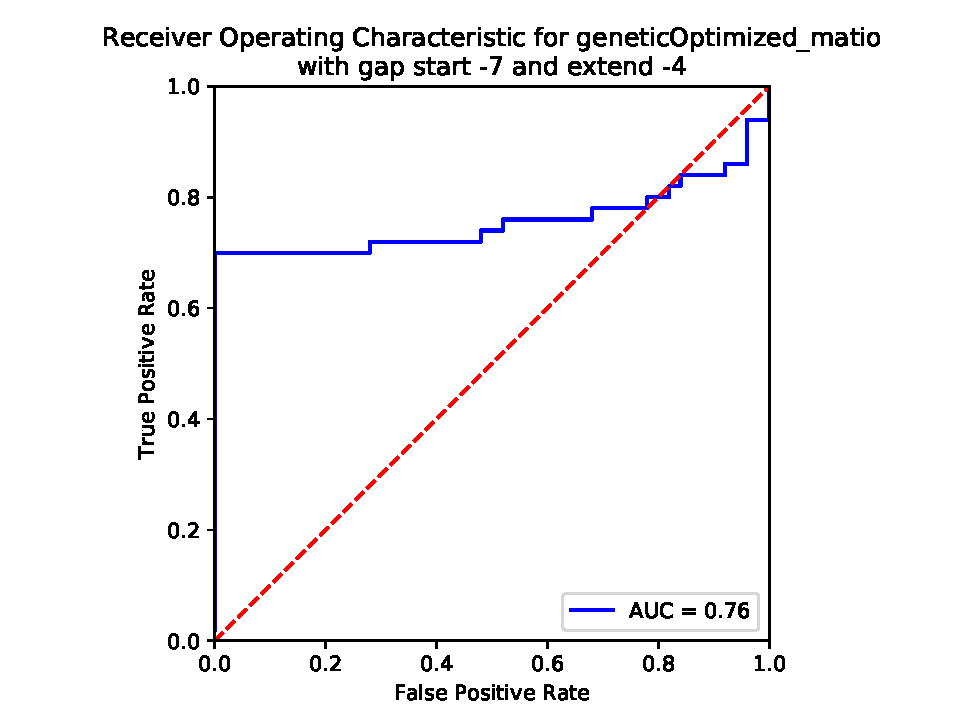
\includegraphics[width=0.5\textwidth]{../BMI203_HW3_alignment/plots/ROC_geneticOptimized_matio.pdf}
\vspace{1em}

Again, realigning and rescoring indicates a much less impressive ROC curve, with an AUC near the original matrix, at 0.71:


\vspace{1em}
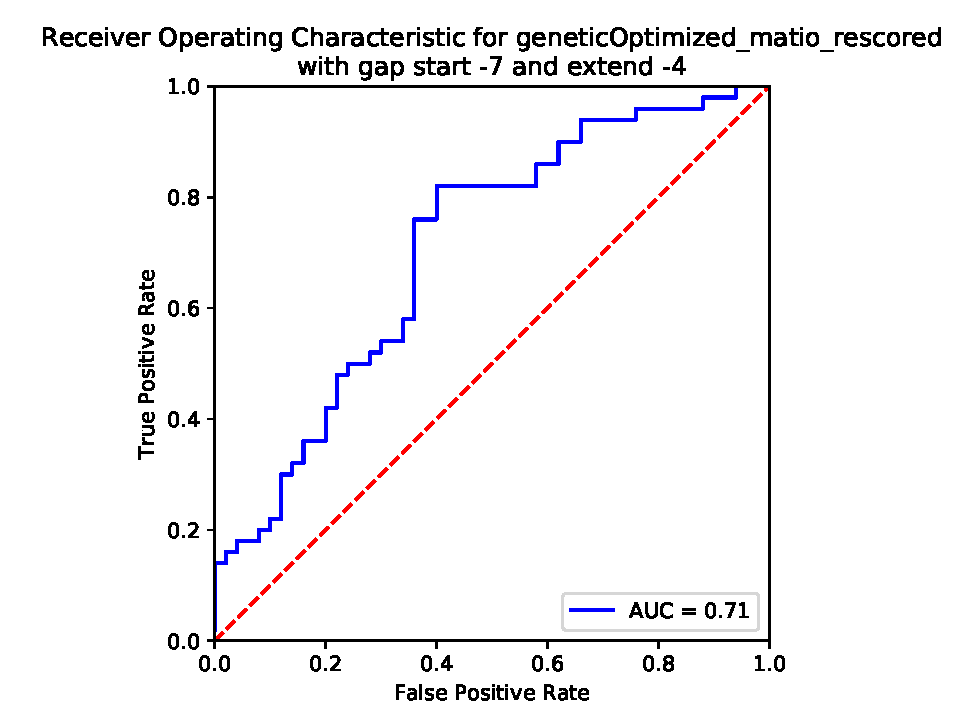
\includegraphics[width=0.5\textwidth]{../BMI203_HW3_alignment/plots/ROC_geneticOptimized_matio_rescored.pdf}
\vspace{1em}

\subsection{Describe your optimization algorithm briefly. How might you improve it?}

I optimized using a genetic algorithm with a population of 100 matrices. In each round of the algorithm, cells of each scoring matrix were mutated with 50\% probability by adding gaussian noise with mean 0 and standard deviation 0.1; then, matrices were scored according to the given objective function, and these scores were renormalized and used as weights for weighted sampling with replacement to form a new generation of matrices. In each step, the population was seeded with 10 matrices with the highest scores we've seen thus far, ensuring that the population stays somewhat diverse and doesn't drift away from identified optima. Iteration stopped after 1000 rounds, or 100 with no new matrices discovered in the top 10.

Empirically, seeding with best-so-far matrices was extremely important to stepping toward optimality; I think it's likely the algorithm would find more optimal matrices more quickly if a larger proportion of the population came from that pool.

I'd also like to do a better job of sampling through matrix space by using perturbations other than cell-independent gaussian noise; I think perturbing rows/columns of the matrix would do a good job of reaching wider into the space in a way that is biologically interpretable ("what if we consider matches/mismatches to this residue more strongly?").

\subsection{What would be required in order to make a convincing case that an optimized matrix will be of general utility and will actually be beneficial for people to use in searching databases?}

To make a convincing case for an optimized matrix, we would need to have a better understanding of its actual predictive power. In order to prove that we're not overfitting our data, we'd want to hold out some data and show that it had good performance on the held-out data. Further, we'd want to validate actual predictions the matrix made by an orthogonal technique.

Finally, substitution matrices are ``tuned'' to find homology across a certain range of evolution distance; we would want to better characterize the range of distances that our optimized matrix is well-suited to work in, so that other researchers could make decisions about whether it would be appropriate to use in their problem.

\end{document}

